\section{Results}
\label{sec:results}

\subsection{The benchmark requires memory (RQ1)}
\label{sec:res_bench}
Episodes last 300 to 1000 control steps with 2--5 picks (Table~\ref{tab:dataset}). A pick, from contact to detachment, occupies only about a dozen frames. In FruitOccludedRipe the gust makes the targeted fruits fully invisible to the front camera. A leaf-hidden fruit is invisible in a median 78\% of the frames in which it still hangs on the tree (Table~\ref{tab:occlusion}), and two-thirds of the hidden fruits are ripe, i.e.\ must be picked. In FruitCount the basket is never in the front view. Neither task can be solved reliably from the current frame: the policy must remember where hidden ripe fruits are and how many fruits it has picked.

\subsection{Picking events from the end-effector-to-fruit distance (RQ2)}
\label{sec:res_events}
Table~\ref{tab:radius} shows event detection from the ground-truth distance as a function of the radius $r$. Precision, recall and F1 are exactly 1.000 for every radius between 1 and 4~cm on both the training set (where $r$ was selected) and the validation set, and every validation episode has the correct pick count. The plateau has a physical explanation. Below the fruit radius (0.5~cm) the gripper does not always come that close and events are missed. Beyond half the inter-fruit spacing (6--10~cm) approaches to neighbouring fruits merge into spurious events. We use $r=3$~cm, in the middle of the plateau. The contact keyframe precedes detachment by a median of 4 frames, and the release keyframe coincides with detachment (median error 0 frames). On the 200 DART-H demonstrations, whose trajectories are perturbed, precision is 0.998, recall 1.000 and the count is exact in 99\% of episodes. Event detection therefore does not depend on smooth expert trajectories.

\begin{table}[t]
\centering
\caption{Event detection versus radius $r$ (tol = 5 mm, ground-truth distance). Train: 200 episodes; validation: 199 episodes with 2--5 picks each. Count: fraction of validation episodes with the exact pick count.}
\label{tab:radius}
\small
\begin{adjustbox}{max width=\textwidth}\begin{tabular}{lcccccccc}
\toprule
 & \multicolumn{3}{c}{Training} & \multicolumn{3}{c}{Validation} & \\
\cmidrule(lr){2-4}\cmidrule(lr){5-7}
$r$ (cm) & P & R & F1 & P & R & F1 & Count\\
\midrule
0.5 & 0.982 & 0.603 & 0.747 & 0.968 & 0.628 & 0.762 & 0.30\\
1 & 1.000 & 1.000 & 1.000 & 1.000 & 1.000 & 1.000 & 1.00\\
2 & 1.000 & 1.000 & 1.000 & 1.000 & 1.000 & 1.000 & 1.00\\
\textbf{3 (used)} & \textbf{1.000} & \textbf{1.000} & \textbf{1.000} & \textbf{1.000} & \textbf{1.000} & \textbf{1.000} & \textbf{1.00}\\
4 & 1.000 & 1.000 & 1.000 & 1.000 & 1.000 & 1.000 & 1.00\\
5 & 0.996 & 1.000 & 0.998 & 0.998 & 1.000 & 0.999 & 0.99\\
6 & 0.971 & 1.000 & 0.985 & 0.962 & 1.000 & 0.981 & 0.91\\
8 & 0.788 & 1.000 & 0.881 & 0.813 & 1.000 & 0.897 & 0.67\\
10 & 0.647 & 1.000 & 0.786 & 0.692 & 1.000 & 0.818 & 0.49\\
\bottomrule
\end{tabular}\end{adjustbox}
\end{table}

\subsection{Robustness to perception error (RQ3)}
\label{sec:res_robust}
Table~\ref{tab:robust} and Fig.~\ref{fig:events} report event detection and memory stability when the validation distance signal is corrupted. The design of the detector makes \emph{independent dropouts} nearly harmless: with 30\% of frames missing, the plain detector still has an F1 of 1.000, because unknown frames inherit the last state. \emph{Systematic bias} of $-1$ to $+2$~cm, as from a miscalibrated depth camera, leaves the pick count exact. \emph{White noise} is the main threat. At 1~cm the plain detector's F1 falls to 0.846 and the count is exact in only 37\% of episodes, because the distance chatters around the threshold. Both filters remove this (F1 0.999, count exact in 99\%). Hysteresis introduces no delay and keeps keyframes closer to their clean positions: keyframe recall is 0.995, against 0.980 for the median filter. It is also more robust to temporally correlated noise (F1 0.953 versus 0.941 at 2~cm), so it is the default deployment detector. The remaining weakness is \emph{long contiguous dropouts} covering an entire approach (30\% of frames in runs averaging 10 frames, F1 0.894--0.913), which motivates combining the front and wrist cameras. From these results we derive an accuracy specification for perception: with hysteresis, a distance error of at most 1.5~cm white noise (F1 0.987) or 2~cm correlated noise (F1 0.953) keeps the event F1 above 0.95.

\begin{table}[t]
\centering
\caption{Robustness of event detection and K4 memory to perturbations of the validation distance signal (5 seeds per level). Each cell: plain / median5 / hysteresis. Keyframe recall: fraction of clean-signal keyframes found within $\pm3$ frames in the perturbed memory.}
\label{tab:robust}
\footnotesize
\begin{adjustbox}{max width=\textwidth}\begin{tabular}{llccc}
\toprule
Perturbation & Level & Event F1 & Count exact & Keyframe recall (K4)\\
\midrule
None & -- & 1.000 / 1.000 / 1.000 & 1.00 / 1.00 / 1.00 & 1.000 / 1.000 / 1.000\\
White noise & 0.5 cm & 0.971 / 1.000 / 1.000 & 0.86 / 1.00 / 1.00 & 0.985 / 0.989 / 0.997\\
White noise & 1 cm & 0.846 / 0.999 / 0.999 & 0.37 / 0.99 / 0.99 & 0.932 / 0.980 / 0.995\\
White noise & 2 cm & 0.635 / 0.969 / 0.947 & 0.03 / 0.85 / 0.78 & 0.846 / 0.966 / 0.958\\
Correlated (OU) & 2 cm & 0.887 / 0.941 / 0.953 & 0.58 / 0.74 / 0.79 & 0.918 / 0.926 / 0.931\\
Independent dropout & 30\% & 1.000 / 1.000 / 0.998 & 1.00 / 1.00 / 0.99 & 0.998 / 0.999 / 0.996\\
Independent dropout & 50\% & 0.996 / 0.996 / 0.988 & 0.98 / 0.98 / 0.94 & 0.982 / 0.987 / 0.973\\
Contiguous dropout & 30\% & 0.913 / 0.913 / 0.894 & 0.62 / 0.62 / 0.55 & 0.882 / 0.901 / 0.867\\
Bias & $-1$ cm & 1.000 / 1.000 / 1.000 & 1.00 / 1.00 / 1.00 & 0.998 / 0.999 / 0.999\\
Bias & $+2$ cm & 1.000 / 1.000 / 1.000 & 1.00 / 1.00 / 1.00 & 1.000 / 1.000 / 1.000\\
\bottomrule
\end{tabular}\end{adjustbox}
\end{table}

\begin{figure}[t]
\centering
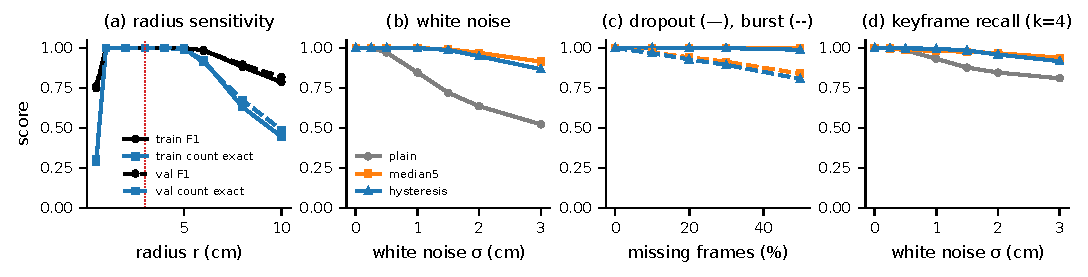
\includegraphics[width=\linewidth]{fig6_event_detection}
\caption{Event detection. (a) F1 and count exact rate versus radius $r$ on training and validation data. (b) F1 versus white-noise level for the plain, median5 and hysteresis detectors. (c) F1 versus the fraction of missing frames, independent (solid) and contiguous (dashed). (d) Recall of K4 memory keyframes ($\pm3$ frames) versus white-noise level.}
\label{fig:events}
\end{figure}

\subsection{What a fixed-budget memory retains (RQ4)}
\label{sec:res_memory}
Table~\ref{tab:coverage} compares memories at the 16-frame budget over 5318 decision points of the validation demonstrations. Figure~\ref{fig:timeline} shows the frames each memory selects in one episode.

\emph{Uniform memory loses picks systematically.} It covers only 57.0\% of the completed picks, and only 43.1\% of decisions can count the picks from memory. Even the most recent pick is covered in only 67.5\% of decisions. A 16-frame uniform memory over a 500-frame episode keeps one frame every 30 frames, while a pick lasts about a dozen frames, so coverage is a matter of chance: random memory reaches 43.2\%, the same order. A recent-frame window is worse still (8.0\%), because it forgets everything before the last 16 frames.

\emph{Forgetting grows with operating time, as the coverage analysis predicts.} Figure~\ref{fig:theory} breaks coverage down by decision time over the 200 validation episodes (7884 decision--pick pairs). At a 16-frame budget, uniform memory covers 97.8\% of completed picks in the first 200 frames, then 56.6\%, 40.8\% and only 26.4\% beyond 600 frames. The most recent pick falls from 97.8\% to 21.7\%: late in an episode, the policy has usually lost sight of the pick it has just made. Equation~(\ref{eq:coverage}) predicts the measured coverage of uniform memory to within 0.012 at every budget (predicted / measured: 0.282 / 0.270 for $B=8$, 0.562 / 0.570 for $B=16$ and 0.882 / 0.883 for $B=32$) and tracks its decay over time (Fig.~\ref{fig:theory}c). The failure is therefore structural, a consequence of sampling geometry, and cannot be tuned away. \pekm\ removes the dependence on time. Both $k=4$ and $k=8$ cover the most recent pick at every decision time (100\%), and $k=8$ covers 94.6\% or more of all completed picks even beyond 600 frames.

\begin{figure}[t]
\centering
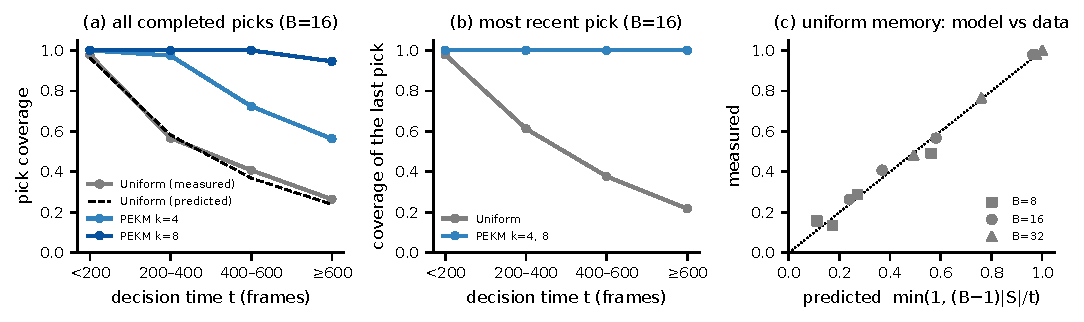
\includegraphics[width=\linewidth]{fig_coverage_theory}
\caption{Time-indexed memory forgets more the longer the robot works. (a) Coverage of all completed picks versus decision time at $B=16$: uniform memory (measured, and predicted by Eq.~(\ref{eq:coverage})) and PEKM. (b) Coverage of the most recent pick. (c) Predicted versus measured coverage of uniform memory for every budget and decision-time bin.}
\label{fig:theory}
\end{figure}

\emph{\pekm\ retains recent picks by construction.} With $k=4$, the last two picks are covered at every decision (100\%), and overall coverage rises to 87.6\%. With $k=8$, coverage reaches 99.6\% and count recoverability 99.2\%, reaching 100\% in FruitOccludedRipe, which has at most three picks. Per task, count recoverability rises from 0.389 (U) to 0.985 (K8) in FruitCount and from 0.485 to 1.000 in FruitOccludedRipe.

\emph{The temporal context is preserved.} The median gap between memory frames grows only from 14 (U) to 17 frames, so the non-event part of the memory keeps nearly the resolution of uniform sampling (Fig.~\ref{fig:coverage}c). The soft variant concentrates more frames near fruits (near-frame fraction 0.265 for $\alpha=1$, six times that of U) and covers older picks evenly. It does so at the cost of the most recent pick (0.814) and of temporal context (median gap 63 frames), which is why hard reservation is the main method.

\emph{Budget efficiency.} Coverage versus budget (Fig.~\ref{fig:coverage}a) shows that K4 with 8 frames (85.9\%) exceeds uniform memory with 16 frames (57.0\%) and approaches uniform memory with 32 frames (88.3\%). K8 with 16 frames (99.6\%) exceeds uniform memory with 32. For field platforms constrained by GPU memory and latency, this means the same event information with a memory two to four times shorter.

\begin{table}[t]
\centering
\caption{Information retained by 16-frame memories (validation, both tasks; 5318 decisions, 7841 decision--pick pairs). Last / 2nd / 3rd: coverage of the most recent, second and third most recent pick. Near: fraction of memory frames with $d_t \le r$. Gap: median gap between memory frames (frames).}
\label{tab:coverage}
\footnotesize
\begin{adjustbox}{max width=\textwidth}\begin{tabular}{lcccccccc}
\toprule
Memory & Event cov. & Run cov. & Count rec. & Last & 2nd & 3rd & Near & Gap\\
\midrule
Uniform (U, K0) & 0.570 & 0.461 & 0.431 & 0.675 & 0.472 & 0.416 & 0.042 & 14\\
Recent & 0.080 & 0.069 & 0.046 & 0.145 & 0.000 & 0.000 & 0.049 & 209\\
Random & 0.432 & 0.364 & 0.329 & 0.533 & 0.351 & 0.231 & 0.040 & 41\\
PEKM $k=2$ & 0.729 & 0.681 & 0.579 & 1.000 & 0.430 & 0.336 & 0.085 & 17\\
\textbf{PEKM $k=4$} & \textbf{0.876} & \textbf{0.875} & \textbf{0.814} & \textbf{1.000} & \textbf{1.000} & 0.136 & 0.110 & 17\\
\textbf{PEKM $k=8$} & \textbf{0.996} & \textbf{0.995} & \textbf{0.992} & \textbf{1.000} & \textbf{1.000} & \textbf{1.000} & 0.123 & 17\\
PEKM $k=12$ & 1.000 & 1.000 & 1.000 & 1.000 & 1.000 & 1.000 & 0.124 & 17\\
PEKM-S $\alpha=0.5$ & 0.878 & 0.854 & 0.756 & 0.811 & 0.982 & 0.948 & 0.153 & 31\\
PEKM-S $\alpha=1$ & 0.897 & 0.873 & 0.770 & 0.814 & 1.000 & 1.000 & 0.265 & 63\\
\bottomrule
\end{tabular}\end{adjustbox}
\end{table}

\begin{figure}[t]
\centering
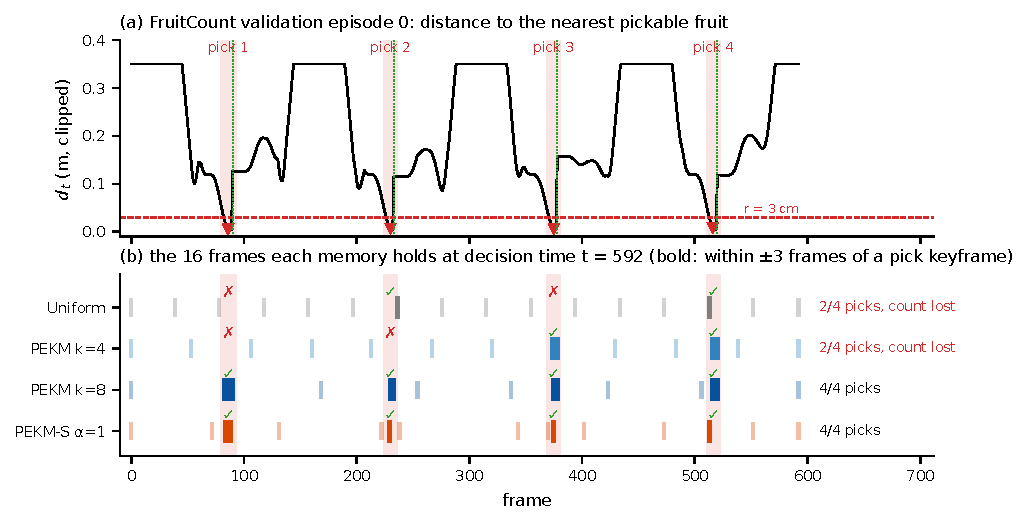
\includegraphics[width=\linewidth]{fig4_memory_timeline}
\caption{Memory timeline of one FruitCount validation episode. Top: the TCP-to-fruit distance $d_t$ with detected events (shaded), contact keyframes (triangles), the radius $r$ (dashed) and fruit detachments (dotted). Bottom: the 16 frames held by uniform memory, PEKM ($k=4$, $k=8$) and PEKM-S ($\alpha=1$) at the last decision.}
\label{fig:timeline}
\end{figure}

\begin{figure}[t]
\centering
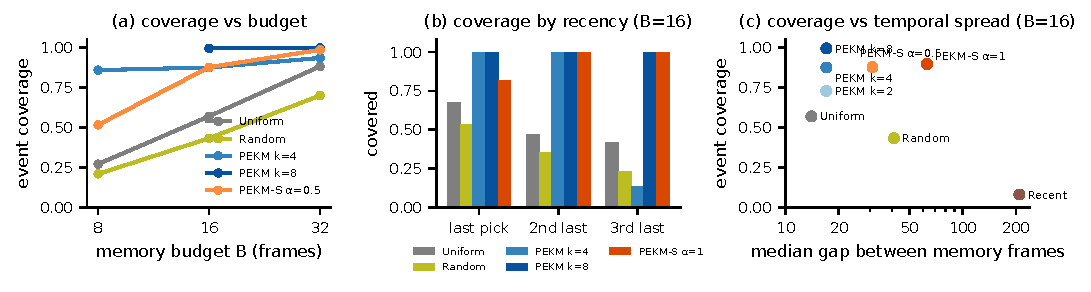
\includegraphics[width=\linewidth]{fig7_memory_coverage}
\caption{Memory coverage. (a) Event coverage versus budget $B$. (b) Coverage of the last three picks at $B=16$. (c) Event coverage versus median gap between memory frames: PEKM raises coverage without sacrificing temporal resolution.}
\label{fig:coverage}
\end{figure}

\subsection{Fruit segmentation with SAM (RQ5)}
\label{sec:res_sam}
Table~\ref{tab:sam} and Fig.~\ref{fig:sam} compare fruit segmentation on 8644 rendered validation images, containing 13{,}424 front-camera and 4877 wrist-camera fruit instances.

\emph{Prompted SAM gives the most accurate masks.} \fdm\ detects fruits with an instance F1 of 0.991 on the front camera and 0.983--0.984 on the wrist camera. Its masks are tighter than those of colour thresholding: the IoU of matched front-camera instances is 0.974--0.978, against 0.945 for HSV. Boundary accuracy matters here because fruit centres are estimated from the back-projected mask (Section~\ref{sec:fdm}), and the resulting anchors are accurate to 0.48~cm (Table~\ref{tab:anchors}). SAM also recovers more partially hidden fruits: front-camera recall is 0.967--0.976 against 0.952 at 25--75\% visibility, and 0.633--0.688 against 0.615 below 25\%. Ripeness is classified correctly for every matched instance by all methods.

\emph{Prompts are essential.} Without prompts, automatic SAM masks filtered by colour and shape (SAM-AUTO) have high precision (0.994--0.996) but miss partially hidden fruits. Front-camera recall drops to 0.57--0.62 at 25--75\% visibility and to 0.21--0.26 below 25\%. SAM-AUTO is also four to seven times slower (395--626~ms per image), because it decodes a dense grid of point prompts.

\emph{A small backbone suffices.} The three backbones have the same F1 (0.991, front camera) and differ by at most 0.004 in IoU, while latency grows from 94~ms (ViT-B) to 195~ms (ViT-L) and 309~ms (ViT-H). The image encoder accounts for more than 90\% of this time. Since anchors are built once per episode and the per-frame vacancy test needs no segmentation (Section~\ref{sec:fdm}), SAM runs once per episode in \fdm, and ViT-B is the practical choice for an embedded platform.

\emph{The remaining gap lies in prompting barely visible fruits.} With ground-truth boxes as prompts, SAM reaches F1 0.999 and a front-camera recall of 0.899 below 25\% visibility. The difference from \fdm\ comes from fruits too small or too occluded to produce a colour component, not from SAM's masks.

\begin{table}[t]
\centering
\caption{Fruit instance segmentation and ripeness on rendered validation images (8644 images; 13{,}424 front and 4877 wrist instances). F1 at IoU $\ge 0.5$. IoU: mean over matched front-camera instances. R (vis.): front-camera recall by visible fraction (418 instances at 25--75\%, 109 below 25\%). Latency: median per front image on one L20 GPU. SAM-AUTO was evaluated on every 5th frame.}
\label{tab:sam}
\footnotesize
\begin{adjustbox}{max width=\textwidth}\begin{tabular}{llccccccc}
\toprule
Method & Backbone & F1 front & F1 wrist & IoU & R (25--75\%) & R ($<$25\%) & Ripeness & ms/img\\
\midrule
HSV thresholds & -- & 0.990 & 0.980 & 0.945 & 0.952 & 0.615 & 1.000 & 1.4\\
SAM-AUTO & ViT-B & 0.937 & 0.983 & 0.979 & 0.573 & 0.263 & 1.000 & 395\\
SAM-AUTO & ViT-H & 0.941 & 0.981 & 0.970 & 0.618 & 0.211 & 1.000 & 626\\
\fdm & ViT-B & \textbf{0.991} & \textbf{0.984} & 0.974 & 0.967 & 0.633 & 1.000 & 94\\
\fdm & ViT-L & \textbf{0.991} & \textbf{0.984} & \textbf{0.978} & \textbf{0.976} & \textbf{0.688} & 1.000 & 195\\
\fdm & ViT-H & \textbf{0.991} & 0.983 & 0.975 & 0.971 & 0.651 & 1.000 & 309\\
\midrule
SAM-GTBOX (upper bound) & ViT-H & 0.999 & 0.999 & 0.980 & 1.000 & 0.899 & 1.000 & --\\
\bottomrule
\end{tabular}\end{adjustbox}
\end{table}

\begin{figure}[t]
\centering
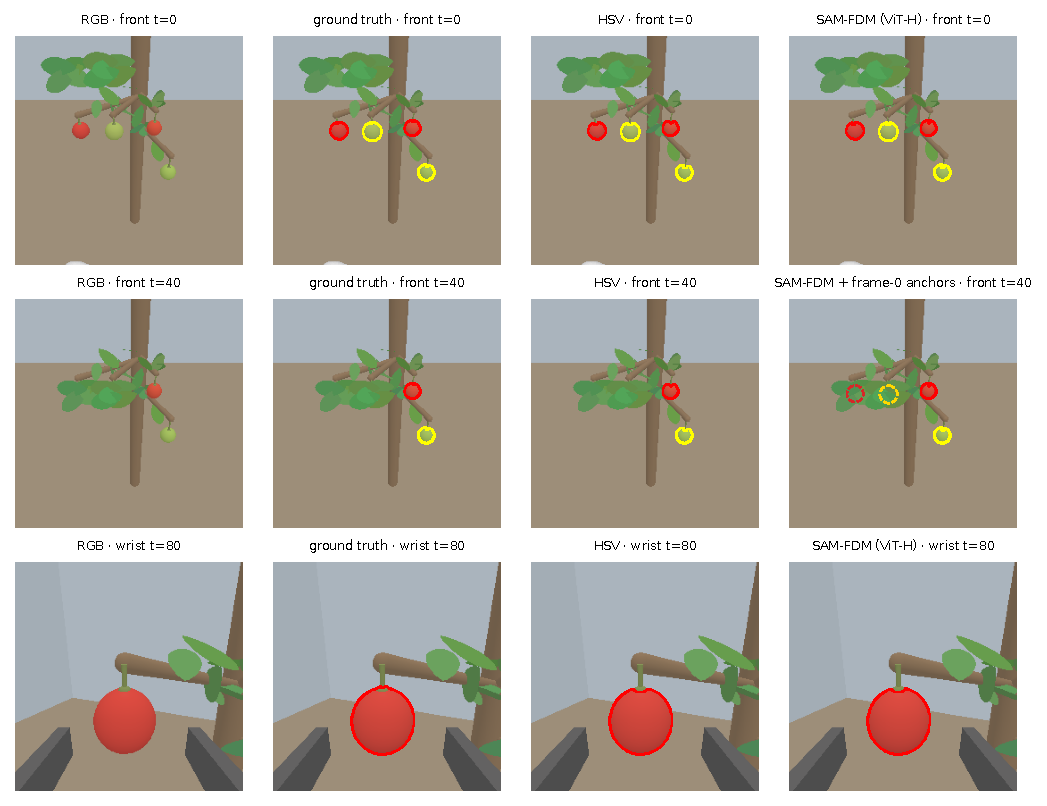
\includegraphics[width=\linewidth]{fig8a_sam_qualitative}\\[2pt]
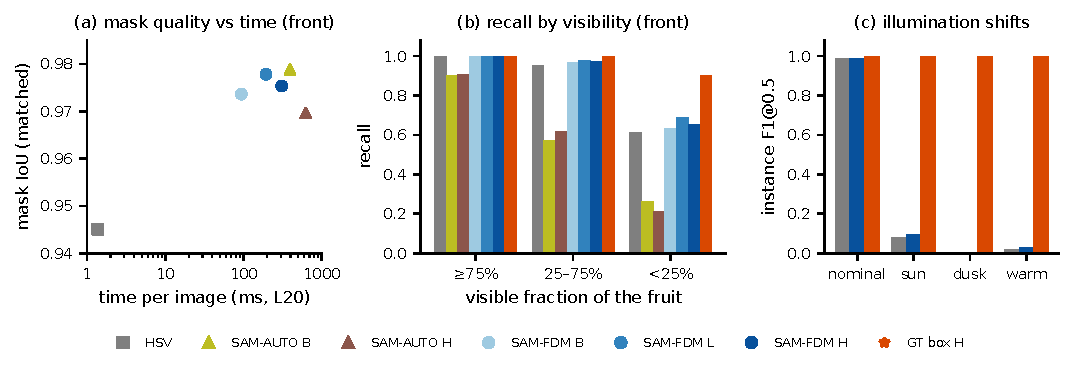
\includegraphics[width=\linewidth]{fig8b_sam_quantitative}
\caption{Fruit segmentation. Top: a FruitOccludedRipe validation episode before the gust (front, $t=0$), after it (front, $t=40$) and at contact (wrist, $t=80$). Columns show the image, ground truth, HSV thresholds and \fdm\ (ViT-H); red contours mark ripe fruits and yellow contours unripe ones. At $t=40$, dashed circles are the frame-0 anchors, which keep the two leaf-hidden fruits in memory. Bottom: (a) mask IoU versus latency; (b) front-camera recall by visible fraction; (c) F1 under illumination shifts.}
\label{fig:sam}
\end{figure}

\emph{Illumination.} To anticipate field conditions, we re-rendered every third frame with three photometric shifts: overcast or dusk ($0.55\,x^{1.2}$), direct sun ($1.35\,x^{0.85}$) and a warm low sun (channel gains 1.12 / 1.00 / 0.80). Colour thresholds were kept as calibrated (Table~\ref{tab:light}). SAM's masks are invariant to these changes: given correct box prompts, F1 stays at 0.999 and IoU at 0.979 under all three conditions. Fixed colour thresholds, by contrast, do not transfer outside their calibration conditions. Their F1 falls below 0.1, and \fdm\ inherits this through its prompts. The analysis locates precisely which component must adapt for field use: the prompt generator. Because prompts are the only input that \fdm\ takes from colour, the thresholds can be replaced by an illumination-normalized colour model or a learned fruit detector without changing SAM, the anchors or the policy. \tbd{Optional: add a row with colour normalization (grey-world white balance + brightness normalization) before thresholding, or a detector trained on randomized-lighting renders, as prompt source.}

\begin{table}[t]
\centering
\caption{Segmentation F1 under illumination shifts (front and wrist cameras together; 6396 instances per shifted condition, 18{,}301 nominal). Colour thresholds as calibrated under nominal lighting. SAM backbone ViT-H.}
\label{tab:light}
\small
\begin{adjustbox}{max width=\textwidth}\begin{tabular}{lcccc}
\toprule
Condition & HSV thresholds & \fdm\ (colour prompts) & SAM-GTBOX F1 & SAM-GTBOX IoU\\
\midrule
Nominal & 0.987 & 0.989 & 0.999 & 0.979\\
Direct sun (bright) & 0.079 & 0.096 & 0.999 & 0.979\\
Overcast / dusk (dark) & 0.000 & 0.000 & 0.999 & 0.979\\
Low sun (warm) & 0.018 & 0.031 & 0.999 & 0.979\\
\bottomrule
\end{tabular}\end{adjustbox}
\end{table}

\subsection{From RGB-D images to event memory (RQ6)}
\label{sec:res_chain}
Tables~\ref{tab:anchors} and~\ref{tab:chain} evaluate the complete chain on the 199 validation episodes. It uses only the recorded front RGB-D frames, forward kinematics and the gripper state, with no simulator ground truth.

\emph{Anchors.} Frame-0 anchors recover 99.8\% of fruits with 99.5\% precision. The median localization error is 0.48~cm (90th percentile 0.58~cm), below a fifth of the fruit radius, and ripeness is classified without error. All 138 ripe fruits that the gust later hides behind leaves have an anchor.

\emph{Distance, events and memory.} The perceived distance $\hat d_t$ has a median error of 0.34~cm in the near range (90th percentile 0.48~cm), well inside the accuracy specification derived in Section~\ref{sec:res_robust}. Events detected from $\hat d_t$ match the ground truth exactly: precision, recall and F1 are 1.000, the count is exact in every episode, the contact lead is 4 frames as with ground truth, and the release error is 0 frames. The resulting PEKM memories recover every ground-truth keyframe (keyframe recall 1.000). The Jaccard similarity is 0.948 for $k=4$ and 0.941 for $k=8$. The remaining differences come from contact frames shifting by one or two frames, which moves the uniform part of the memory; no event information is lost. Consumer-grade depth noise leaves all results unchanged.

\emph{Spatial memory before occlusion is necessary.} When anchors are built after the gust (frame 29), anchor recall drops to 0.783, and to 0.568 in FruitOccludedRipe. None of the 138 leaf-hidden ripe fruits receives an anchor. Event recall in FruitOccludedRipe falls to 0.450, and \emph{no} FruitOccludedRipe episode has the correct pick count (0.00, against 1.00 with frame-0 anchors). FruitCount, which has no foliage occlusion, is unaffected. Perceiving a fruit while it is visible and remembering where it is is therefore a precondition for remembering that it was picked.

\emph{Grasp evidence closes the visual blind spot.} With depth vacancy alone, the arm and the carried fruit occlude the anchor's pixels during carrying, so detachment is confirmed only after the arm leaves: the release keyframe is late by a median of 16 frames, and the memory Jaccard drops to 0.685. Adding the gripper-holding cue, a proprioceptive signal available at almost no cost, removes the delay.

\emph{Anchors are more reliable than per-frame detection.} Without anchors, the fruit being carried in the gripper is still detected as the nearest fruit. The release error grows to 52 frames, and spurious events appear (precision 0.821, count exact in 62\% of episodes; 0.759 and 46\% in FruitCount, where carried fruits repeatedly disappear and reappear). Hysteresis suppresses some of them (precision 0.942), but the memory Jaccard remains 0.421. Figure~\ref{fig:chain} illustrates these behaviours on one episode.

\begin{table}[t]
\centering
\caption{Fruit anchors from \fdm\ (ViT-H) on 199 validation episodes, matched to the true fruit positions at frame 0 (5 cm gate). Hidden ripe: fraction of ripe fruits later hidden by leaves that have an anchor ($n=138$).}
\label{tab:anchors}
\small
\begin{adjustbox}{max width=\textwidth}\begin{tabular}{lccccc}
\toprule
Anchors & Recall & Precision & Error med / p90 (cm) & Ripeness acc. & Hidden ripe\\
\midrule
Frame 0 (before gust, ours) & 0.998 & 0.995 & 0.48 / 0.58 & 1.000 & \textbf{1.000}\\
Frame 0 + depth noise & 0.998 & 0.995 & 0.45 / 0.56 & 1.000 & 1.000\\
Frame 29 (after gust) & 0.783 & 0.993 & 0.49 / 0.58 & 1.000 & 0.000\\
\bottomrule
\end{tabular}\end{adjustbox}
\end{table}

\begin{table}[t]
\centering
\caption{Events and memory from perceived distances (199 validation episodes; plain detector, hysteresis in parentheses). Dist.\ err.: median / 90th-percentile error of $\hat d_t$ where $d_t \le 10$ cm. Rel.\ err.: median error of the release keyframe (frames). Jaccard and KF recall: agreement of the K4 memory with the memory computed from ground truth. For K8, Jaccard is 0.941 / 0.941 / 0.660 / 0.730 / 0.363 and KF recall 1.000 / 1.000 / 0.847 / 0.882 / 0.782 for the rows below GT.}
\label{tab:chain}
\footnotesize
\begin{adjustbox}{max width=\textwidth}\begin{tabular}{lcccccccc}
\toprule
Distance source & Dist.\ err.\ (cm) & P & R & F1 & Count & Rel.\ err. & Jaccard & KF recall\\
\midrule
GT (upper bound) & 0 / 0 & 1.000 & 1.000 & 1.000 & 1.00 & 0 & 1.000 & 1.000\\
\textbf{\fdm\ (ours)} & \textbf{0.34 / 0.48} & \textbf{1.000} & \textbf{1.000} & \textbf{1.000} & \textbf{1.00} & \textbf{0} & \textbf{0.948} & \textbf{1.000}\\
\fdm\ + depth noise & 0.31 / 0.46 & 1.000 & 1.000 & 1.000 & 1.00 & 0 & 0.948 & 1.000\\
Depth-only & 0.39 / 10.76 & 1.000 & 1.000 & 1.000 & 1.00 & 16 & 0.685 & 0.845\\
Post-gust anchors & 0.39 / -- & 1.000 & 0.743 & 0.853 & 0.50 & 0 & 0.741 & 0.880\\
Per-frame & 0.39 / 12.79 & 0.821 (0.942) & 1.000 & 0.902 (0.970) & 0.62 (0.85) & 52 & 0.421 & 0.755\\
\bottomrule
\end{tabular}\end{adjustbox}
\end{table}

\begin{figure}[t]
\centering
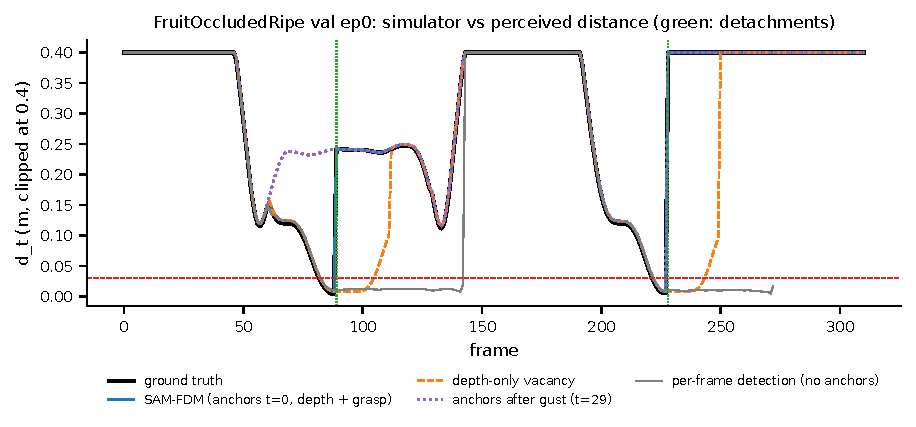
\includegraphics[width=\linewidth]{fig_e6_perceived_distance}
\caption{Perceived versus ground-truth distance in one FruitOccludedRipe episode. Vertical lines mark fruit detachments. \fdm\ follows the ground truth. Depth-only vacancy confirms detachment late, post-gust anchors miss the hidden ripe fruit, and per-frame detection tracks the carried fruit.}
\label{fig:chain}
\end{figure}

\subsection{Closed-loop harvesting (RQ7)}
\label{sec:res_closed}
Table~\ref{tab:closed} reports closed-loop results on validation episodes 50--99 (150 trials per task and condition). \tbd{Main results text after the sealed evaluation: success rates of K0/K4/K8 per task with paired differences, 95\% CIs and Holm-adjusted p-values; process metrics (completion, over-pick in FruitCount, wrong-pick in FruitOccludedRipe, drops, steps); stratification by quota $N$ (2 / 3 / 4--5); validity gates (engineering errors, frame-selection audit).}

\begin{table}[t]
\centering
\caption{Closed-loop harvesting on validation episodes 50--99 (3 seeds; 150 trials per cell). Paired differences with 95\% bootstrap CIs; Holm-adjusted p-values over the primary family.}
\label{tab:closed}
\footnotesize
\begin{adjustbox}{max width=\textwidth}\begin{tabular}{llcccccc}
\toprule
Task & Memory & Success & Completion & Over-/wrong-pick & Drop & Steps & $\Delta$ vs K0 [95\% CI]\\
\midrule
FruitCount & K0 (uniform) & \tbd{} & \tbd{} & \tbd{} & \tbd{} & \tbd{} & --\\
 & K4 (PEKM) & \tbd{} & \tbd{} & \tbd{} & \tbd{} & \tbd{} & \tbd{}\\
 & K8 (PEKM) & \tbd{} & \tbd{} & \tbd{} & \tbd{} & \tbd{} & \tbd{}\\
FruitOccludedRipe & K0 (uniform) & \tbd{} & \tbd{} & \tbd{} & \tbd{} & \tbd{} & --\\
 & K4 (PEKM) & \tbd{} & \tbd{} & \tbd{} & \tbd{} & \tbd{} & \tbd{}\\
 & K8 (PEKM) & \tbd{} & \tbd{} & \tbd{} & \tbd{} & \tbd{} & \tbd{}\\
\bottomrule
\end{tabular}\end{adjustbox}
\end{table}

\subsection{Ablations and counterfactual controls}
\label{sec:res_ablation}
Table~\ref{tab:ablation} lists the test-time ablations, evaluated with the K4 policy under the same paired protocol. \tbd{Results text: (a) keyframe cap; (b) budget; (c) radius 1/3/5 cm; (d) hard vs soft selection; (e) signal source GT / SAM-FDM / noisy GT; (f) counterfactual controls EVU, EVR and EVA; (g) keyframe composition (contact only / release only / both).}

\begin{table}[t]
\centering
\caption{Ablations (test-time variants of the K4 policy unless noted; paired differences to the default configuration).}
\label{tab:ablation}
\footnotesize
\begin{adjustbox}{max width=\textwidth}\begin{tabular}{llcc}
\toprule
Factor & Setting & FruitCount $\Delta$ & FruitOccludedRipe $\Delta$\\
\midrule
Keyframe cap $k$ (trained) & 0 / 4 / 8 & \tbd{} & \tbd{}\\
Radius $r$ & 1 / 3 / 5 cm & \tbd{} & \tbd{}\\
Selection & hard (PEKM) / soft (PEKM-S, $\alpha=0.5$) & \tbd{} & \tbd{}\\
Signal source & GT / \fdm\ / GT + 1 cm noise & \tbd{} & \tbd{}\\
Counterfactual & EV / EVU / EVR / EVA & \tbd{} & \tbd{}\\
Keyframes & contact / release / both & \tbd{} & \tbd{}\\
Training data & clean (C0) / clean + DART-H (K0) & \tbd{} & \tbd{}\\
\bottomrule
\end{tabular}\end{adjustbox}
\end{table}

\subsection{Open-loop accuracy, closed-loop drift and DART-H (RQ8)}
\label{sec:res_dart}
Table~\ref{tab:openloop} evaluates a policy trained on clean demonstrations in open loop, predicting actions at the demonstrated states. TCP errors at the end of a 16-step chunk are 1.7--2.4~cm (median), and 0.7--1.1~cm during the near-fruit phase, an order of magnitude below the motion within a chunk (about 10~cm). The gripper open/close direction agrees with the demonstration in 98--99.5\% of decisions. Training and validation errors are nearly identical: the policy has learned the demonstrations and generalizes to unseen layouts. In closed loop, however, small deviations accumulate and move the robot into states that clean demonstrations do not cover. This is the covariate shift that DART-H targets. Its perturbations (median TCP displacement 2.5~cm) match the scale of these errors. \tbd{Closed-loop C0 vs K0 comparison and the time of first departure from the demonstrated distribution.}

\begin{table}[t]
\centering
\caption{Open-loop (teacher-forced) accuracy of a uniform-memory policy trained on clean demonstrations (10 episodes per set). TCP error at horizons 1, 8 and 16 of the action chunk; near: horizon 16 while $d_t \le 10$ cm.}
\label{tab:openloop}
\small
\begin{adjustbox}{max width=\textwidth}\begin{tabular}{llccc}
\toprule
Set & Task & TCP error h1 / h8 / h16 (cm) & Near h16 (cm) & Gripper agreement\\
\midrule
Train & FruitCount & 0.44 / 1.23 / 1.83 & 0.75 & 99.5\%\\
Train & FruitOccludedRipe & 0.42 / 1.25 / 1.66 & 0.70 & 99.2\%\\
Validation & FruitCount & 0.51 / 1.37 / 2.38 & 1.14 & 98.0\%\\
Validation & FruitOccludedRipe & 0.40 / 1.32 / 1.75 & 0.78 & 98.9\%\\
\bottomrule
\end{tabular}\end{adjustbox}
\end{table}

\subsection{Memory content matters for VLA policies}
\label{sec:res_general}
To show that the frames a VLA policy remembers affect its actions, and not only an offline coverage metric, we evaluated the base policy on a general manipulation-memory benchmark (\tbd{cite RoboMME}) under sealed protocols (Table~\ref{tab:general}). Removing the history memory collapses success on a pattern-recall task from 66.7\% to 1.7\%. Halving the budget from 32 to 16 frames reduces it from 64.4\% to 26.7\%. Replacing a single memory slot changes the expert's action loss consistently: the ranking of slots is reproducible with a reliability of 0.97--0.99 across four tasks. Within a fixed budget, the choice of frames therefore has a substantial effect on the policy. This is the premise of \pekm.

\begin{table}[t]
\centering
\caption{Memory ablations of the base VLA on a general manipulation-memory benchmark (paired bootstrap, Holm-adjusted).}
\label{tab:general}
\footnotesize
\begin{adjustbox}{max width=\textwidth}\begin{tabular}{p{4.6cm}p{7.6cm}}
\toprule
Intervention & Result\\
\midrule
No history memory (pattern-recall task) & 66.7\% $\rightarrow$ 1.7\% ($-65.0$ pp, 95\% CI [$-81.7$, $-46.7$], $p<0.001$)\\
No memory (video-swap task) & $-11.7$ pp (95\% CI [$-20.0$, $-3.3$], $p=0.006$)\\
Budget 32 $\rightarrow$ 16 frames (pattern recall) & 64.4\% $\rightarrow$ 26.7\% ($-37.8$ pp, $p<0.001$)\\
Single-slot replacement (counterfactual action loss) & Slot ranking reliability 0.97--0.99 over four tasks; cross-fitted relative gain 2.5--12.4\%\\
\bottomrule
\end{tabular}\end{adjustbox}
\end{table}

\subsection{Run-time cost}
\label{sec:res_cost}
\pekm\ adds negligible computation. At $t=1000$ frames, one selection takes 117~$\mu$s (median; 99th percentile 125~$\mu$s) on a CPU core, against 39~$\mu$s for uniform sampling, which is negligible compared with one VLA inference (\tbd{VLA inference latency, ms}). Because the budget is unchanged, the memory footprint and inference cost of the policy are identical to the uniform baseline. \fdm\ segments an image in 94 / 195 / 309~ms with ViT-B / ViT-L / ViT-H on one L20 GPU, dominated by the image encoder. It runs SAM only when anchors are built, once per episode. The per-frame work, projecting a handful of anchors and reading their depth and the gripper state, takes well under a millisecond.
